% !TEX encoding = UTF-8
% !TEX TS-program = pdflatex
% !TEX root = ../Tesi.tex

%************************************************

%************************************************

\section{Infarinatura Neural Networks}

\subsubsection{Neurone}
Il neurone è l'elemento basilare del sistema nervoso, tanto che può essere considerato l'unità di calcolo primaria alla base della mente umana. In figura \ref{img:neurone} è mostrata la rappresentazione biologica di un neurone ed il modello matematico ad esso ispirato: ogni neurone riceve in input il segnale dai suoi dendriti e, una volta elaborato, produce un segnale di output lungo il suo unico assone, che una volta diramatosi lo collega ai neuroni successivi attraverso le sinapsi.

\begin{figure}[htb]
	\centering
	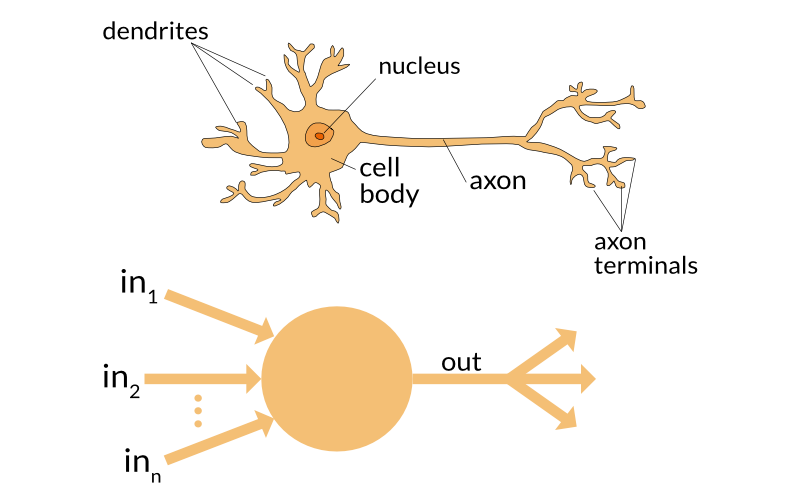
\includegraphics[width = 100mm]{images/neuron.png}
	\caption{Dalla rappresentazione biologica di un neurone al modello matematico.}
	\label{img:neurone}
\end{figure}

Questa attività biologica può essere rappresentata da un modello matematico nel quale i segnali che viaggiano attraverso gli assoni interagiscono con i dendriti dei neuroni con i quali sono collegati. La modifica delle sinapsi (i pesi $w$), rappresenta l'apprendimento. Nel modello base i dendriti portano il segnale al corpo della cellula, dove sono sommati: se il risultato di questa somma supera una certa soglia, il neurone attiva l'impulso attraverso l'assone. Tale somma viene attivata da una funzione di attivazione. In altre parole, ogni neurone esegue un prodotto vettoriale tra i suoi input e il suo set di pesi, somma un termine di distorsione (bias) e infine applica una funzione di attivazione non lineare. La funzione di attivazione deve necessariamente essere non lineare, in caso contrario la rete neurale si ridurrebbe ad un modello lineare generalizzato.

\begin{figure}[htb]
	\centering
	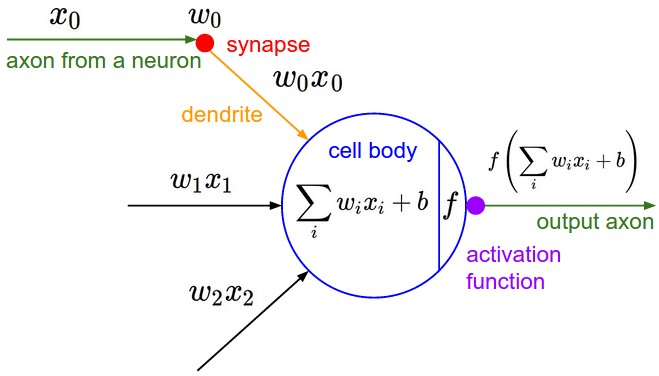
\includegraphics[width = 100mm]{images/neuron_model.jpeg}
	\caption{Modello matematico di neurone.}
	\label{img:modello_neurone}
\end{figure}

Nella figura è rappresentata una semplice rete neurale con 4 predittori $x_j$, un singolo strato nascosto composto da 5 neuroni calcolato: $x^{(1)} = \sigma(Wx^{(0)} + b)$ layer 1 dove $\sigma$ è la funzione di attivazione, $W$ è il set di pesi, $x^{(0)}$ è il vettore di input e $b$ è il bias. L'output è data da una singola unità $y = \sigma(Wx^{(1)} + b)$.

L'idea di base è quella che ogni neurone apprenda una semplice funzione binaria. Lo strato finale è caratterizzato anch'esso dalla presenza di un vettore di pesi e di una funzione di output, che generalmente corrisponde alla funzione identità in problemi di regressione, o alla softmax in problemi di classificazione. Cambiando il numero di strati e dei neuroni, le reti neurali possono essere considerate come approssimatori universali di funzioni \cite{hornik1989multilayer}.

\begin{figure}[htb]
	\centering
	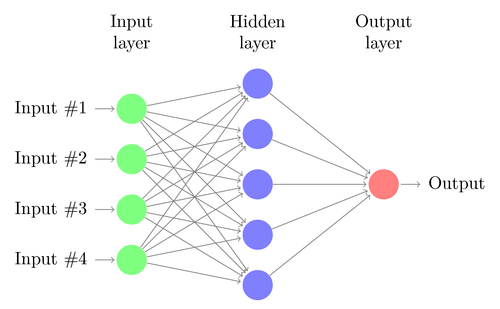
\includegraphics[width = 100mm]{images/onehidden.png}
	\caption{Multilayer perceptron.}
	\label{img:multilayer_perceptron}
\end{figure}

Il termine Deep Learning prende nome dalla profondità che caratterizza le reti neurali multistrato, dove con profondità ci si riferisce al numero di strati nascosti presenti. Le reti deep vengono infatti chiamate anche MLP, ovvero MultiLayer Perceptron \cite{goodfellow2016deep}.


\subsubsection{Layer}
I neuroni sono organizzati in layer, moduli di elaborazione dati che possono essere considerati come un filtro per i dati. Alcuni dati entrano, e ne escono in una forma più utile. Nello specifico, i layer estraggono rappresentazioni che, auspicabilmente, dovrebbero essere più significative per il problema in questione. La maggior parte dell'apprendimento consiste nel concatenare insieme semplici livelli che implementeranno una forma di astrazione progressiva dei dati, fino ad una rappresentazione di alto livello in grado di portare a termine il task.

\subsubsection{Activation function}
Lo scopo della funzione di attivazione è quello di aggiungere non-linearità nella rete, permettendo di modellare output che non variano linearmente al variare dei predittori. Questo significa che l'output non può essere rappresentato da una combinazione lineare dell'input. Senza non-linearità, anche aggiungendo diversi strati nascosti in una rete, questi risulterebbero equivalenti ad uno strato solo (single-layer Perceptron).

\subsubsection{Sigmoid}
Inizialmente la più utilizzata, la funzione sigmoide è stata progressivamente accantonata negli ultimi anni per via di alcune problematiche che comporta a livello pratico.

La prima e più importante è quella relativa alla dissolvenza del gradiente in seguito alla saturazione dei neuroni, ossia quei neuroni che presentano valori di output agli estremi del codominio della funzione di attivazione, in questo caso $(0, 1)$. Tale saturazione diventa problematica durante la fase di addestramento della rete (Back Propagation, sezione \ref{backprop}), in quanto il gradiente locale assume valori prossimi allo zero, conducendo così all'annullamento del gradiente globale \cite{glorot2010understanding}. In pratica si ha un flusso utile del gradiente solo per valori di input che rimangono all'interno di una zona di sicurezza, cioè nei dintorni dello zero.

Il secondo problema deriva invece dal fatto che gli output della funzione sigmoide non sono centrati intorno allo zero \cite{lecun1998gradient}. Si consideri il caso in cui tutti gli input di un nodo sono positivi. L'aggiornamento dei pesi entranti in un determinato neurone avviene in modo proporzionale all'errore in quel nodo (uno scalare) ed il vettore di input. Se tutte le componenti del vettore in input sono positive, tutti gli aggiornamenti dei pesi che arrivano in quel neurone avranno lo stesso segno (il segno dell'errore) e i pesi quindi saranno o tutti incrementati o tutti diminuiti. Se il vettore di pesi in considerazione deve cambiare direzione, questo può avvenire solamente dopo diverse iterazioni di aggiornamento (zigzagando), rallentando così l'apprendimento. Questo si comporta inoltre come una fonte di bias sistematico per i neuroni nello strato successivo della rete. Per aggirare questo problema è stata introdotta come funzione di attivazione la Tangente Iperbolica in quanto funzione dispari. L'apprendimento con Backpropagation con funzioni dispari porta ad una convergenza più veloce rispetto ad un processo con funzioni non simmetriche \cite{haykin2004comprehensive}.

Il terzo e ultimo difetto della funzione sigmoide è che l'operazione esponenziale al denominatore è molto costosa dal punto dal punto di vista computazionale, soprattutto rispetto alle alternative che verranno presentate di seguito.

\begin{figure}[htb]
	\centering
	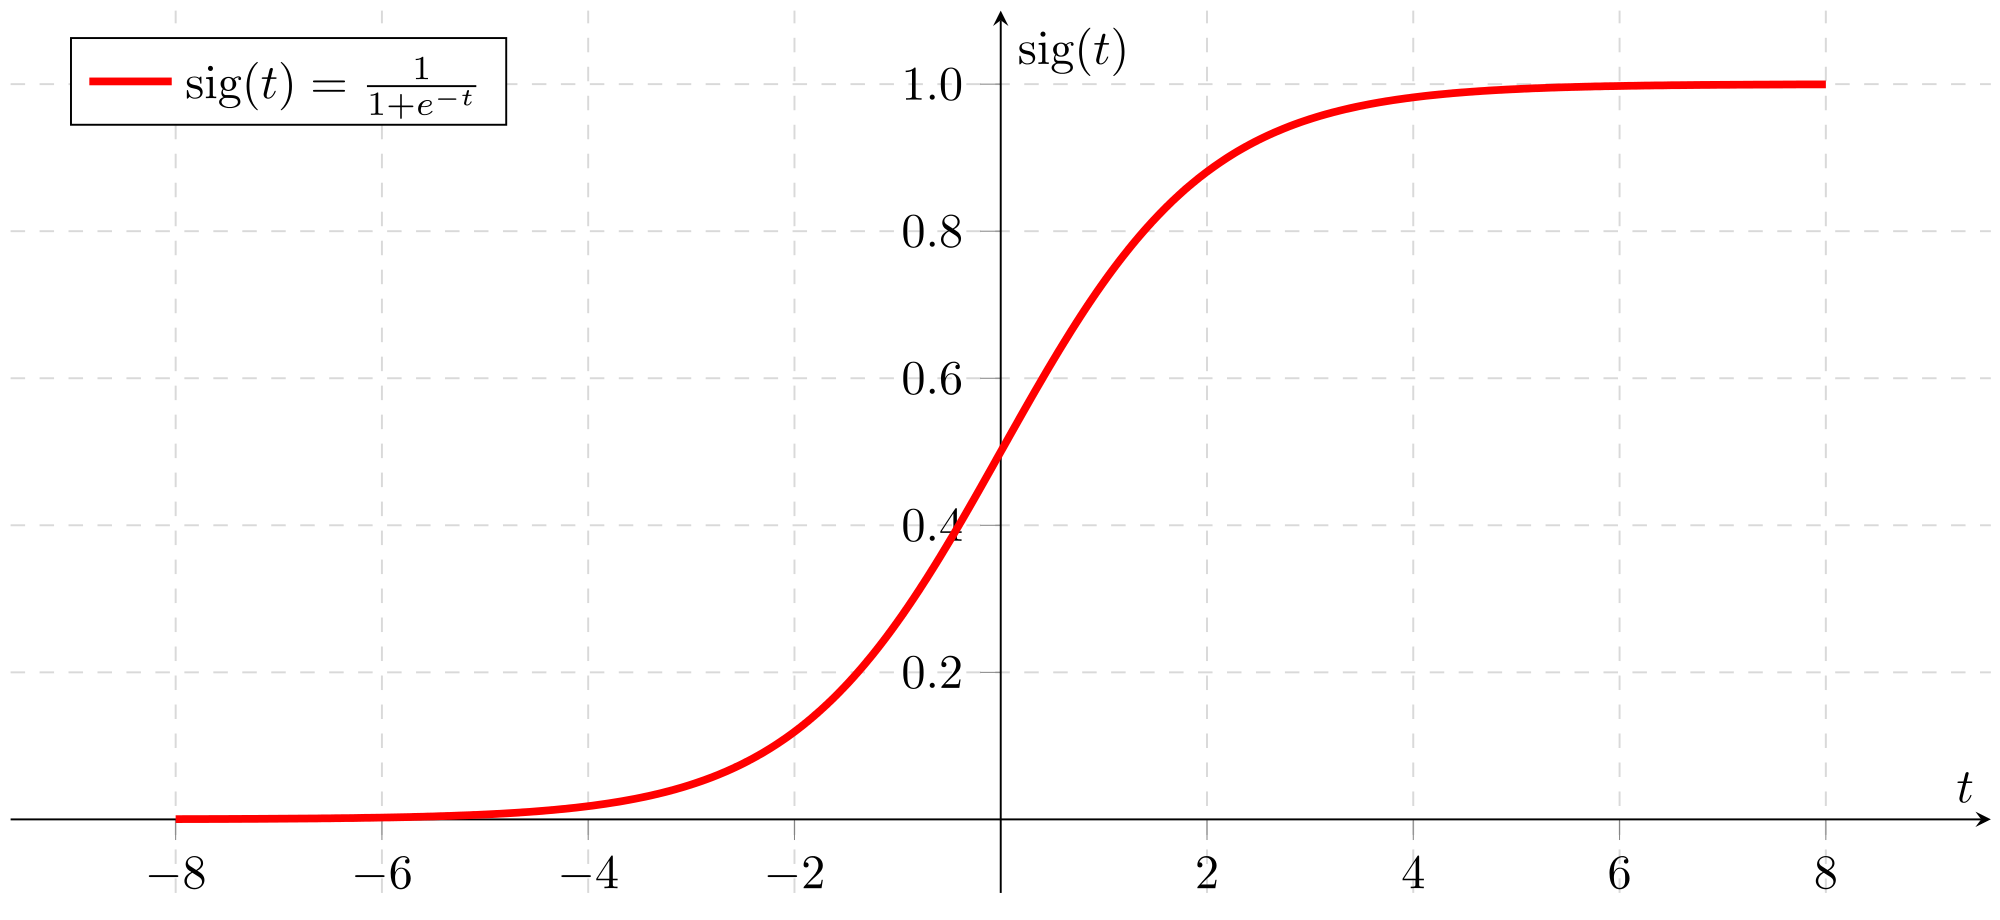
\includegraphics[width = 100mm]{images/sigmoid.png}
	\caption{Funzione sigmoide.}
	\label{img:sigmoid}
\end{figure}

\subsubsection{TanH}
Il problema degli output non centrati sullo zero \cite{haykin2004comprehensive} della sigmoide può essere risolto ricorrendo all'utilizzo della tangente iperbolica, la quale presenta codominio $(−1, 1)$ centrato sull'origine degli assi. Tuttavia, rimane il problema della saturazione dei neuroni, anzi viene addirittura accentuato, dal momento che la zona di sicurezza risulta ancora più ristretta.

\begin{figure}[htb]
	\centering
	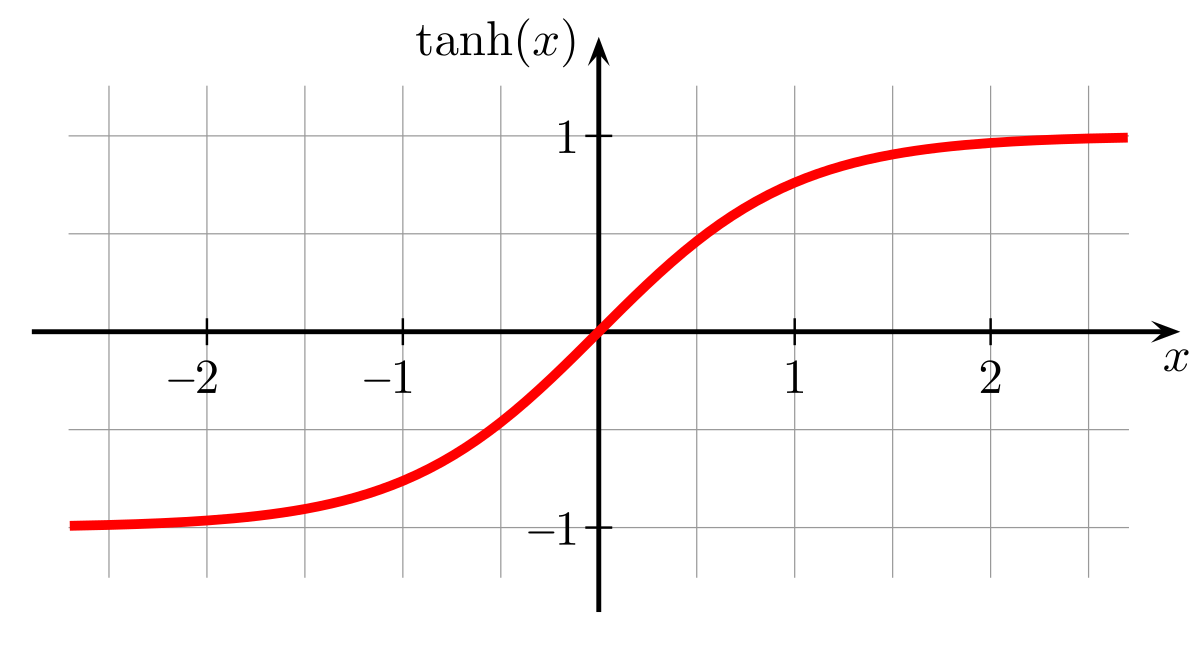
\includegraphics[width = 100mm]{images/tanh.png}
	\caption{Funzione TanH.}
	\label{img:tanh}
\end{figure}

\subsubsection{ReLU}
La Rectified Linear Unit (ReLU) è diventata popolare negli ultimi anni per via dell'incremento prestazionale che offre nel processo di convergenza: velocizza infatti di circa 6 volte la discesa del gradiente rispetto alle alternative viste finora. Questo risultato è da attribuire in larga parte al fatto che la ReLU risolve il problema della dissolvenza del gradiente \cite{glorot2010understanding}, non andando a saturare i neuroni. Durante la fase di Back Propagation (sezione \ref{backprop}) infatti, se il gradiente calcolato fino a quel punto è positivo questo viene semplicemente lasciato passare, perchè la derivata locale per il quale viene moltiplicato è pari ad uno. Eventuali problemi sorgono invece quando il gradiente accumulato ha segno negativo, in quanto questo viene azzerato (le derivata locale è nulla lungo tutto il semiasse negativo) con la conseguenza che i pesi non vengono aggiornati. Fortunatamente questo problema può essere alleviato attraverso l'utilizzo di un algoritmo SGD (batch size maggiori di 1) \cite{ioffe2015batch}: considerando più dati alla volta c'è infatti la speranza che non tutti gli input del batch provochino l'azzeramento del gradiente, tenendo così in vita il processo di apprendimento del neurone. Al contrario, se per ogni osservazione la ReLU riceve valori negativi, allora il neurone "muore", e non c'è speranza che i pesi vengano aggiornati. Valori elevati del learning rate amplificano questo problema, dal momento che cambiamenti più consistenti dei pesi si traducono in una maggiore probabilità che questi affondino nella "zona morta".
\begin{figure}[htb]
	\centering
	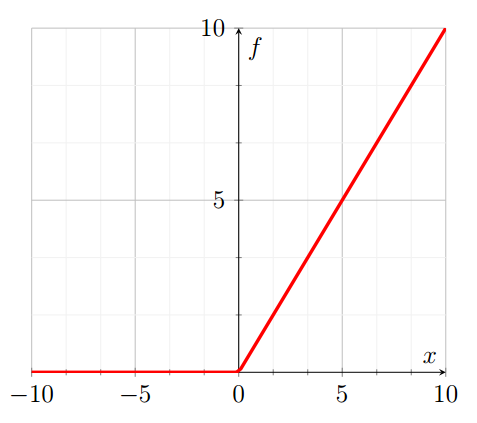
\includegraphics[width = 100mm]{images/relu.png}
	\caption{Funzione ReLU.}
	\label{img:relu}
\end{figure}

\subsection{Training}

\subsubsection{Loss function}
%A loss function: how the network will be able to measure its performance on the training data, and thus how it will be able to steer itself in the right direction.

\subsubsection{Optimizer}
%An optimizer—The mechanism through which the network will update itself based on the data it sees and its loss function.

\subsubsection{Metrics}
%Metrics to monitor during training and testing—Here, we’ll only care about accu- racy (the fraction of the images that were correctly classified).



\subsubsection{BackPropagation}
\label{backprop}
L'apprendimento dei pesi di una rete neurale non risulta un compito semplice, trattandosi come abbiamo visto di una complessa funzione gerarchica $f(x;W)$ del vettore di input $x$ e della collezione di pesi $W$.  Innanzitutto è necessario scegliere opportunamente le funzioni di attivazione in modo che tale funzione risulti differenziabile. Si tratta quindi di risolvere una funzione di perdita $L[y, f(x)]$.

Le funzioni di perdita sono generalmente convesse in $f$, ma non negli elementi di $W$, con la conseguenza che ci troviamo a dover risolvere un problema di minimizzazione su una superficie che presenta una grande quantità di minimi locali. Una soluzione è quella di effettuare più stime dello stesso modello con differenti inizializzazioni dei parametri, per scegliere infine quello che risulta essere migliore. Una procedura di questo tipo può però richiedere molto tempo, che spesso non è disponibile, pertanto generalmente ci si tende ad accontentare di buoni minimi locali.

I principali metodi utilizzati sono basati sulla tecnica della discesa del gradiente, la cui implementazione in questo contesto prende il nome di Back-Propagation \cite{werbos1974beyond}, in virtù del fatto che lo scarto registrato in corrispondenza di un certo dato viene fatto propagare all'indietro nella rete per ottenere le formule di aggiornamento dei coefficienti. Dal momento che $f(x;W)$ è definita come una composizione di funzioni a partire dai valori di input della rete, gli elementi di $W$ sono disponibili solo in successione (quella degli strati) e pertanto la differenziazione del gradiente seguirà la regola della catena (chain rule).

Data una generica osservazione $(x, y)$ l'algoritmo di back-propagation prevede di effettuare un primo passo in avanti lungo l'intera rete (feed-forward step) e salvare le attivazioni che si creano ad ogni nodo $x_{l}^{(k)}$ di ogni strato $l$, incluso quello di output. La responsabilità di ogni nodo nella previsione del vero valore di $y$ viene quindi misurata attraverso il calcolo di un termine d'errore $\delta_{l}^{(k)}$. Nel caso delle attivazioni terminali $x_{l}^{(k)}$ il calcolo di tali errori è semplice: coincide infatti con i residui o loro trasformazioni, in base a come viene definita la funzione di perdita. Per le attivazioni degli strati intermedi $\delta_{l}^{(k)}$ viene calcolato invece come somma pesata dei termini d'errore dei nodi che utilizzano $x_{l}^{(k)}$ come input.

Una volta calcolato il gradiente è possibile procedere con l'aggiornamento del sistema dei pesi. Il calcolo del gradiente ci fornisce la direzione lungo la quale la superficie da minimizzare è più ripida, ma nessuna informazione circa la lunghezza del passo che dovremmo compiere. Tale quantità viene denominata learning-rate e costituisce l'iperparametro più importante da regolare in una rete neurale: valori alti portano ad una convergenza più veloce ma sono rischiosi dal momento che potrebbero saltare il minimo ottimale o fluttuare intorno ad esso, mentre valori bassi sono responsabili di una convergenza lenta e possono comportare il blocco dell'algoritmo in un minimo locale non ottimale.

\subsubsection{Stochastic Gradient Descent}
Esistono alcune varianti dell'algoritmo di discesa del gradiente che differiscono nella quantità di dati utilizzati nel calcolo del gradiente prima di effettuare l'aggiornamento dei parametri. Quella classica utilizza ad ogni iterazione l'intero dataset. Tuttavia, può spesso risultare più efficiente processare piccole quantità di dati (batch) per volta, generalmente campionate in maniera casuale, da qui il nome Stochastic Gradient Descent (Bottou, 2010). Tale scelta è obbligata quando le dimensioni del dataset sono tali da non poter essere caricato in memoria. Valori estremi del batch come n oppure 1 possono causare problemi rispettivamente di calcoli ridondanti (il gradiente viene ricalcolato sempre su osservazioni simili prima dell'aggiornamento) e di fluttuazioni della funzione da minimizzare, a causa di aggiornamenti troppo frequenti e variabili, essendo basati sulla singola osservazione. Di conseguenza si tendono a scegliere valori intermedi. Indipendentemente dal numero di iterazioni e dalla dimensione del batch prescelta, ogni volta che tutte le osservazioni del dataset vengono utilizzate per il calcolo del gradiente si dice che viene completata un'epoca.

\subsubsection{Ottimizzazione discesa del Gradiente}
Ci sono alcune modifiche che possono essere apportate all'algoritmo di discesa del gradiente per migliorarne le performance, legate soprattutto al learning rate. Possono sorgere complicazioni invece quando si tratta di minimizzare funzione non convesse, con il rischio di rimanere intrappolati in minimi locali non ottimali. Di seguito verranno presentati alcuni algoritmi di ottimizzazione che mirano alla risoluzione di questo tipo di problematiche.

\begin{itemize}
    \item \textbf{Momentum}: SGD presenta alcune difficoltà in prossimità di aree dove la superficie presenta una curvatura molto più accentuata in una direzione rispetto all'altra (Sutton, 1986). In questo scenario infatti l'algoritmo tende ad oscillare lungo il versante più ripido, rallentando così la convergenza verso il minimo locale ottimale. Momentum \cite{qian1999momentum} è un metodo che aiuta ad accelerare la discesa del gradiente verso la direzione corretta, smorzando l'effetto indotto dalle oscillazioni. Tale risultato si ottiene aggiungendo al termine di aggiornamento corrente una frazione gamma del vettore di aggiornamento precedente.
    
    \item \textbf{AdaGrad}: Momentum permette di adattare i nostri aggiornamenti in relazione alla superficie da minimizzare velocizzando così la convergenza, ma non fa nessuna distinzione circa l'importanza dei parametri, trattandoli tutti allo stesso modo. Adagrad \cite{duchi2011adaptive} è un algoritmo di ottimizzazione nato proprio con questo scopo: adattare il learning rate ai parametri, permettendo così di effettuare aggiornamenti più consistenti in corrispondenza dei parametri relativi alle features meno frequenti, e viceversa. In particolare, nella sua regola di aggiornamento, Adagrad utilizza un alpha differente per ogni parametro ad ogni iterazione, modificando quest'ultimo sulla base dei gradienti passati che sono stati calcolati per lo specifico parametro. Uno dei più grandi benefici di Adagrad consiste nell'eliminare la necessità di settare manualmente il learning rate: è necessario impostare solamente il valore iniziale. D'altra parte, il suo punto debole è invece l'accumulo eccessivo del quadrato dei gradienti al denominatore, che comporta un'esagerata e progressiva riduzione del learning rate, il quale tende a diventare infinitamente piccolo, al punto tale che l'algoritmo non è più in grado di acquisire nuova informazione, arrestando così il processo di convergenza.
\end{itemize}




\subsection{Prediction}
Spiegato il framework di base nel quale il Deep Learning rientra, nella prossima sezione parleremo delle reti Convolutional, le quali introducono un nuovo tipo di layer, più adatto all'elaborazione delle immagini in quanto in grado di imparare pattern locali invece di pattern globali.


\section{Convolutional Neural Networks}
Un'immagine è composta da pixel. Nel modello RGB, ogni pixel ha tre colori elementi, rosso, verde e blu. Più comunemente ogni elemento può variare da 0 (nessun colore) a 255 (saturazione completa) di valore. In computer vision, un'immagine è una matrice di pixel a tre strati, dove ogni strato è una matrice bidimensionale che rappresenta il rosso, il verde o il blu valori dei pixel \ref{rgb_tensor}.


\begin{figure}[htb]
	\centering
	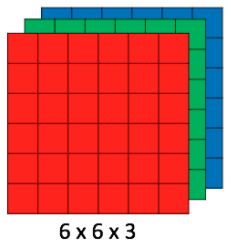
\includegraphics[width = 40mm]{images/rgb_tensor.png}
	\caption{Tensore di un immagine rgb.}
	\label{rgb_tensor}
\end{figure}


Le Convolutional Neural Networks (CNN) sono una classe di reti neurali e una delle più comuni architetture di apprendimento profondo per il riconoscimento delle immagini. Il modello prende un'immagine di input, essa passa attraverso una serie di strati convoluzionali finalizzati all'estrazione di pattern visivi che saranno dati in input agli strati successivi fully connected, i quali produrranno la classificazione.


Il termine "convoluzione" si riferisce alla composizione matematica di due funzioni per formare una terza funzione. Nel contesto delle CNN, viene applicato uno strato convoluzionale (chiamato filtro o kernel) ai dati di input per produrre una feature map.

\begin{figure}[htb]
	\centering
	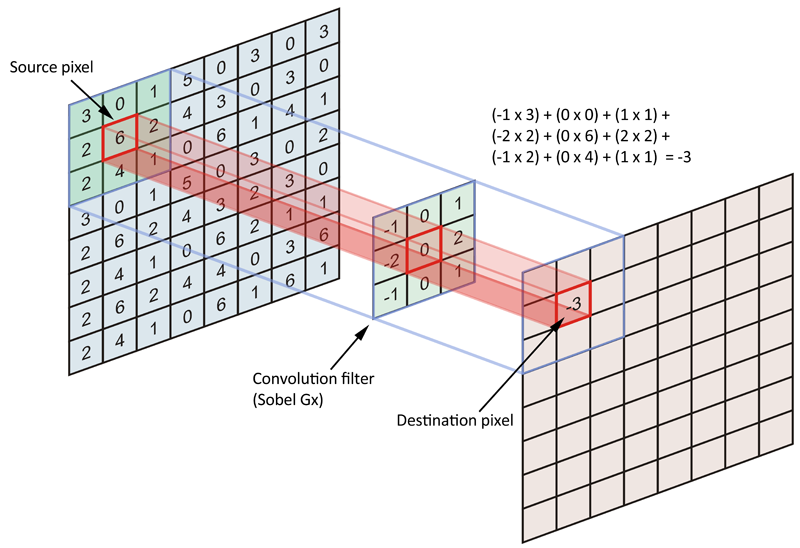
\includegraphics[width = 100mm]{images/conv1.png}
	\caption{Applicazione della funzione di convoluzione.}
	\label{conv1}
\end{figure}

In \ref{conv1}, viene effettuata una moltiplicazione scalare tra una matrice di dimensioni 3x3 (kernel) ed una porzione di dimensioni 3x3 della della immagine in input. Gli elementi della matrice risultante vengono sommati e la somma è il valore di output sulla feature map risultante. Il filtro viene fatto scorrere sulla matrice di input fino a completare la feature map. 

Molteplici filtri sono applicati producendo più feature map che verranno concatenate lungo la terza dimensione, producendo un tensore tridimensionale. Ci sono altri due concetti importanti negli strati convoluzionali: stride e padding. Lo stride è un valore numerico che rappresenta il numero di pixel che un kernel scorre sull'input matrice. Il padding  rappresenta il numero di strati pixel da aggiungere alla matrice bidimensionale dell'immagine in modo da poter applicare l'operatore di convoluzione anche in prossimità dei bordi.


\subsection{Pooling}
I pooling layer sono responsabili della riduzione della dimensionalità delle feature map, in particolare l'altezza e la larghezza, preservando la profondità. Questo porta a due vantaggi, riduce la potenza di calcolo richiesta ed estrae le feature dominanti 

Il max pooling restituisce il valore massimo degli elementi nella parte di immagine coperta dal kernel, mentre l'average pooling restituisce il valore medio come in figura \ref{pooling}.

\begin{figure}[H]
	\centering
	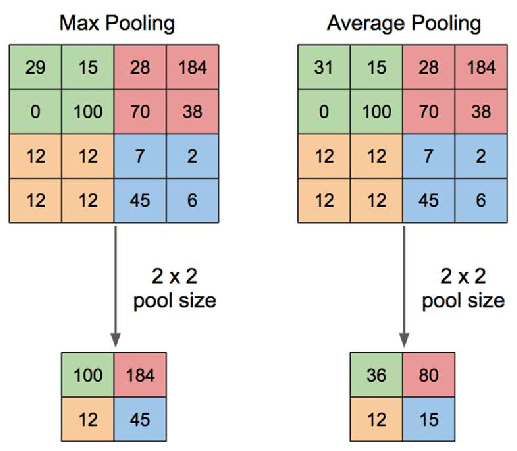
\includegraphics[width = 100mm]{images/pooling.png}
	\caption{Differenza tra max e averag pooling..}
	\label{pooling}
\end{figure}

\subsection{Fully connected}
Gli strati fully connected sono finalizzati alla classificazione vera e propria. La matrice in input, con le feature estratte dai layer di convoluzione, viene appiattita in un vettore e viene fatta passare  attraverso strati di neuroni fully connected. L'output dell'ultimo strato è un vettore N-dimensionale, dove N è il numero di classi tra le quali la CNN deve scegliere. Ogni numero in questo vettore ndimensionale rappresenta la probabilità che l'immagine appartenga a ciascuno certa classe.



\subsection{Object detection}

La capacità di identificare gli oggetti presenti in un'immagine è un compito naturale per gli esseri umani, farlo fare ad una macchina però si è dimostrato estremamente difficile. Questo compito è notoriamente suddiviso in due sotto problemi, la classificazione e la localizzazione. La classificazione etichetta l'oggetto dominante presente una data immagine con una delle classi che ha imparato a riconoscere. Il compito più impegnativo è la localizzazione: oltre a etichettare l'oggetto dominante questo deve anche essere localizzato, solitamente determinando un riquadro intorno alla regione dell'immagine occupata dall'oggetto (Bounding Box). La difficoltà aumenta ulteriormente se consideriamo che in un immagine possono essere etichettati e rilevati più oggetti, della stessa categoria o no. Questo compito di etichettare e rilevare è chiamato \textbf{Object Detection}. Ad oggi è un campo di ricerca ampio e molto attivo, di seguito una breve panoramica sui progressi recenti.

\begin{figure}[htb]
	\centering
	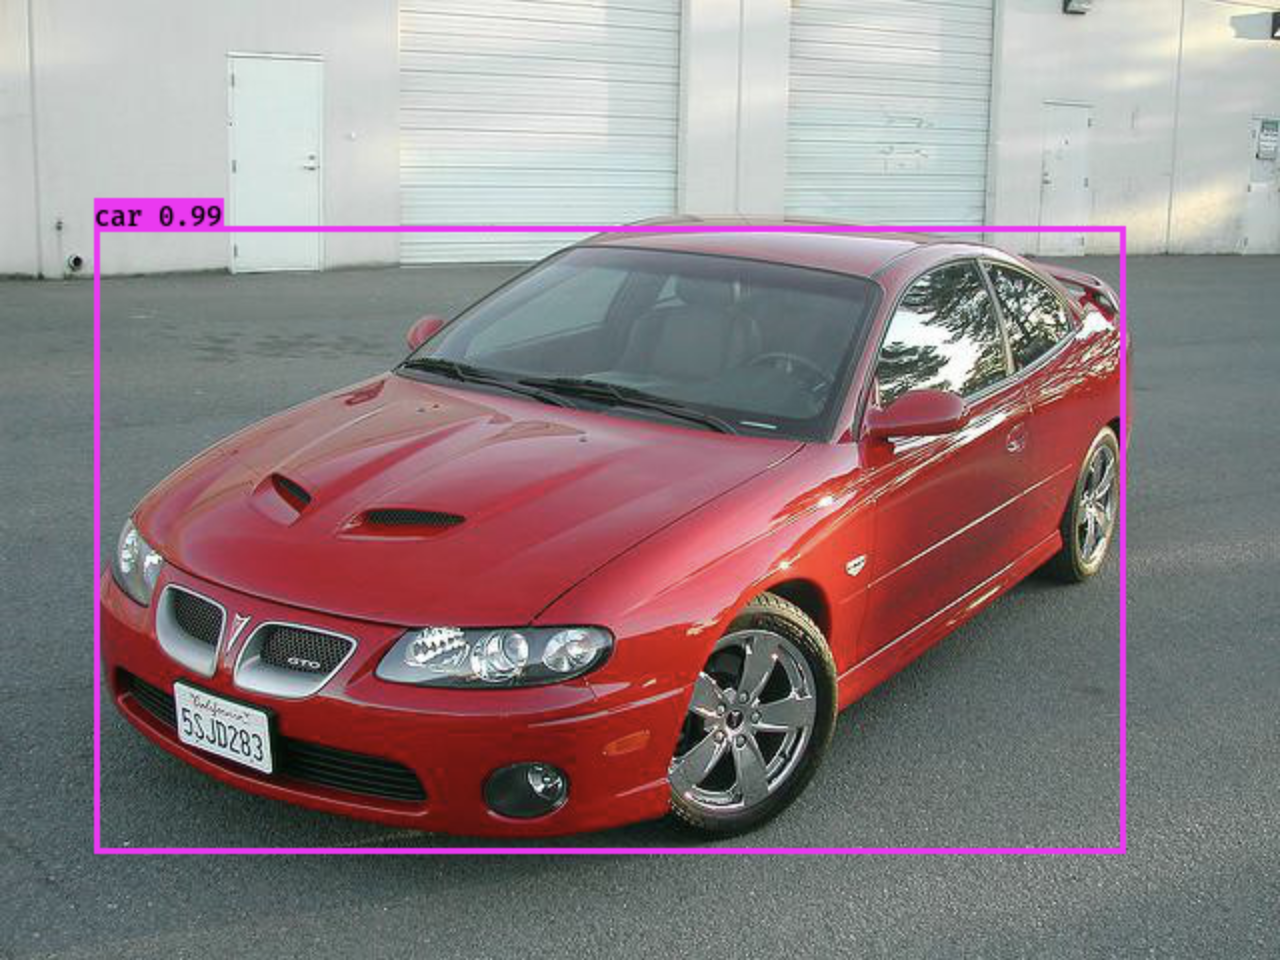
\includegraphics[width = 100mm]{images/car_od.png}
	\caption{Riconoscimento e localizzazione, task di object detection.}
	\label{car_od}
\end{figure}

Un buon mezzo per giudicare quanto sia vicina a risolvere il problema è stata la competizione \textit{PASCAL Visual Object Challenge (VOC)} e successivamente \textit{ImageNet large scale visual recognition challenge (ILSVRC)} \cite{russakovsky2015imagenet}. Pascal VOC è iniziato nel 2005 e si è svolto ogni anno fino al 2012. Nei primi anni la maggior parte delle proposte utilizzava tecniche di bag-of-visual-word basati su feature visuali costruite ad-hoc come SIFT \cite{sift} e HOG \cite{hog}.

Nel 2012, la sfida ha visto un grande miglioramento delle prestazioni, quando Krizhevsky et al. \cite{krizhevsky2012imagenet} ha introdotto per la prima volta in una rete neurale convoluzionale (Convolutional Neural Netwrok o CNN).

Per la classificazione delle immagini, l'output della CNN è un vettore n-dimensionale che contiene la probabilità che l'oggetto appartenga ad una delle possibili classi. Per la localizzazione la rete aagiunge un task di regressione delle coordinate della bounding box, come introdotto in \cite{krizhevsky2012imagenet}.

Il grande svantaggio di questo approccio è che non è applicabile se il numero di bounding box non è noto in precedenza. I primi tentativi di risolvere questo problema furono la divisione dell'immagine in sotto porzioni (attraverso una sliding window) e l'applicazione della classificazione e la localizzazione ad ogni parte dell'immagine (a scale diverse). Questo approccio con sliding window) è ovviamente estremamente costoso a causa dell'enorme spazio di ricerca. Per ridurre il numero di predizioni necessarie alla rete, una soluzione è stata l'applicazione di una griglia più larga, in modo da ridurre il numero di predizioni necessarie ma andando a trovare bounding box solamnete in posizioni predefinite. Idealmente, si vorrebbe avere una serie iniziale di \textit{regioni} in qualche modo proposte da poter essere valutate. Questo è stato l'approccio introdotto con successo da Girshick et al. \cite{girshick2014rich} nel loro lavoro chiamato \textbf{R-CNN}. Per generare le le regioni da proporre, hanno utilizzato l'algoritmo \textit{Selective search} \cite{uijlings2013selective} che genera regioni sulla base di un approccio di segmentazione gerarchica.

% breve su fast e faster cnn, breve su yolo e poi anche su <nuovo algoritmo> ?

L'approccio descritto finora si basa su due step \ref{2step_od},, una parte di generazione delle regioni, indipendente dalle classi, e per ogni regione trovata, una classificazione:  la rete non guarda al completo immagine, ma scansiona molte regioni (passo di region proposal), cercando di capire quale regione sia una buona candidata a contenere un oggetto. Lo svantaggio di tali metodi è la necessità di utilizzare una CNN per lo step di classificazione all'interno di ciascuna regione. Poiché si potrebbe voler rilevare oggetti di dimensioni diverse, questo approccio porta alla generazione di molte regioni, portano a lunghi tempi di calcolo e non possono essere eseguite tempo reale. La precisione di queste tecniche, tuttavia, è molto alta.

\begin{figure}[htb]
	\centering
	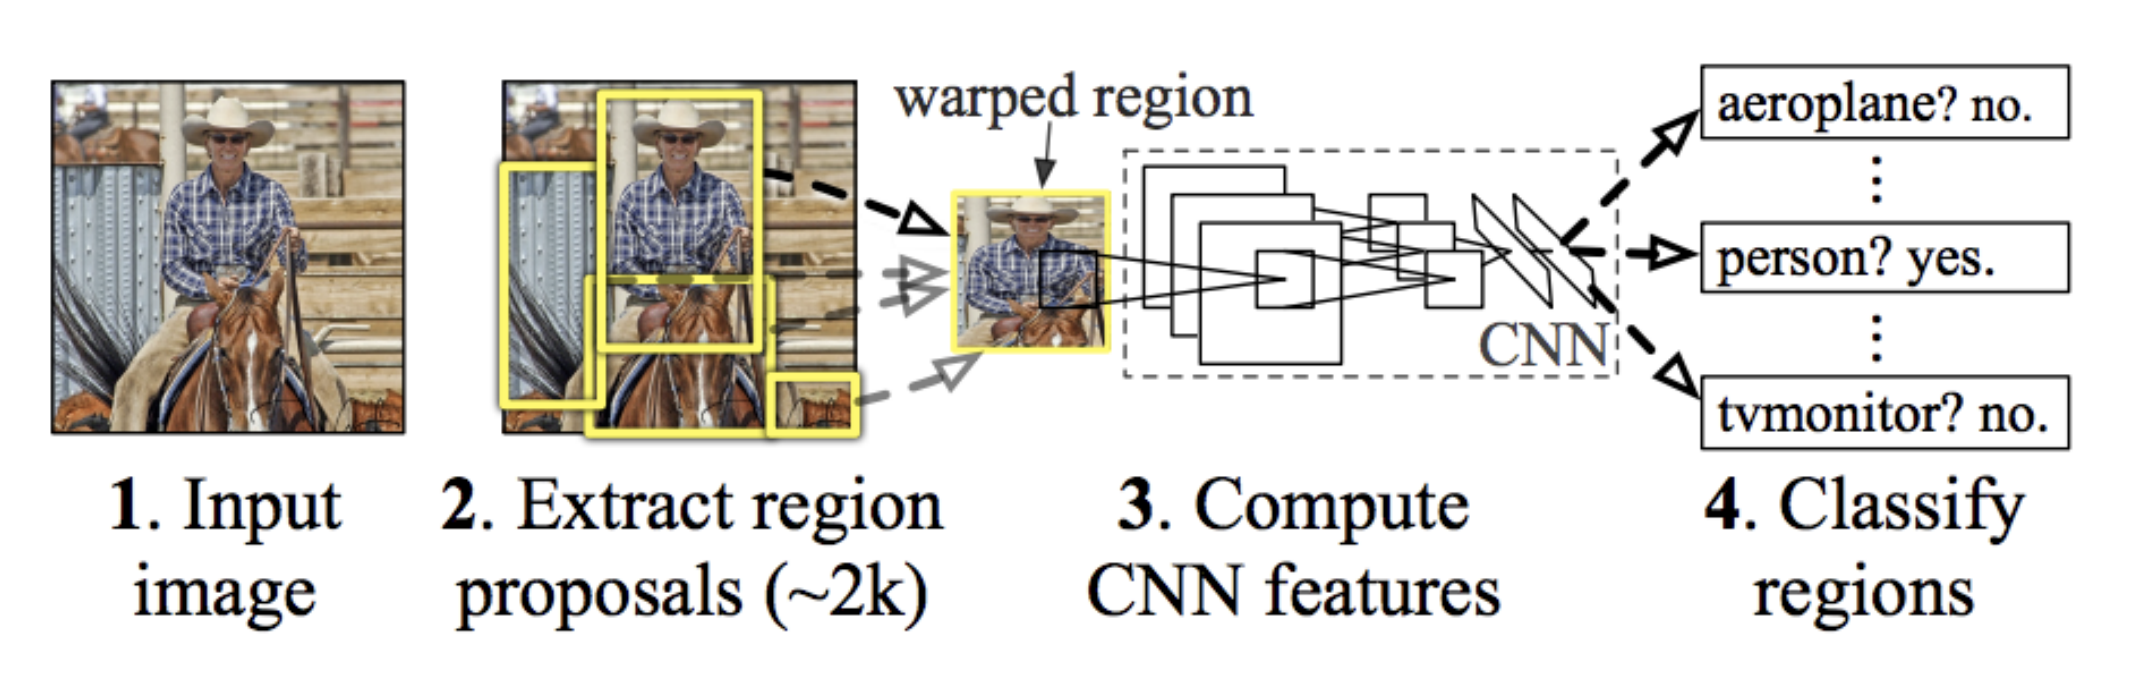
\includegraphics[width = 120mm]{images/2step_od.png}
	\caption{Object Detection con Fast-RCNN.}
	\label{2step_od}
\end{figure}


La svolta è arrivata quando è stato introdotto un approccio ad una sola passata in \cite{redmon2016you}.

YOLO - You Only Look Once - è una convolutional neural network basata sul classificatore Darknet, arrivato la sua terza versione YOLO v3. Sia YOLO che Darknet sono stati inizialmente progettati e sviluppato da Joseph Redmon \cite{redmon2016you}.

Questo approccio differisce dalle tecniche basate sulla region proposal viste sopra. In un'unica passata una Convolutional Neural Network predice le bounding box e le probabilità per ogni classe all'interno della bounding box: l'immagine di input è divisa in una griglia SxS. Se il centro di un oggetto cade in una cella della griglia, quella cella è responsabile del rilevamento di quell'oggetto. Ogni cella della griglia produce B bounding box con la probabilità per ogni classe. Il numero completo di bounding box per immagine è 98 che supera 2000 da R-CNN ma è anche migliore di 300 da Faster R-CNN. Quindi, un ottimo vantaggio è che YOLO può eseguire in tempo reale è dunque S×S×( C+5*B ) (5 perchè 4 coord + obj score).

\begin{figure}[htb]
	\centering
	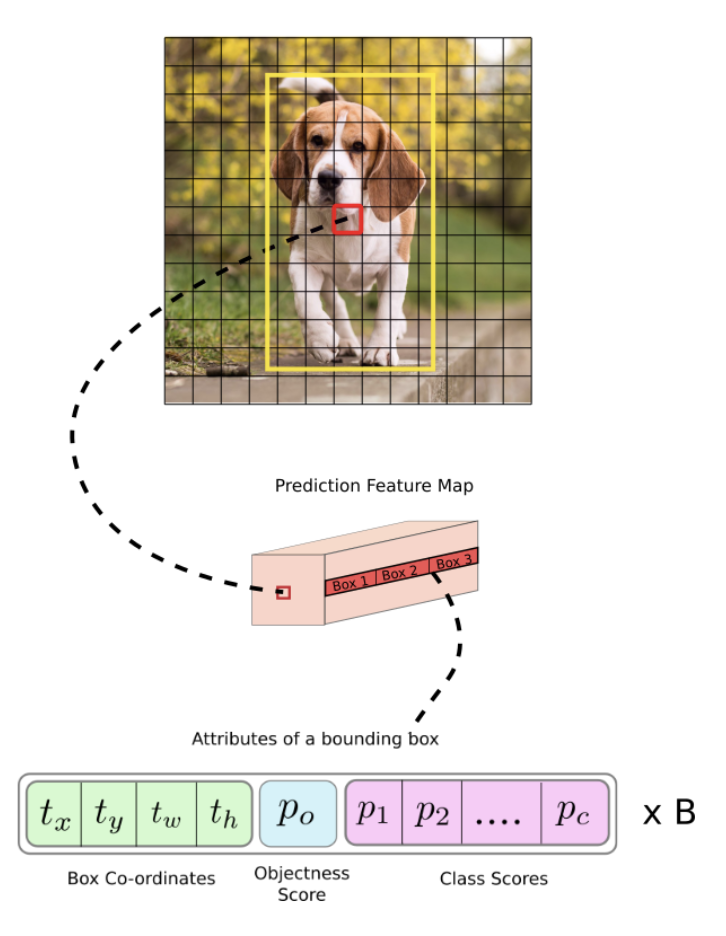
\includegraphics[width = 120mm]{images/yolo_od.png}
	\caption{YOLO.}
	\label{yolo_od}
\end{figure}



\subsection{Segmentation}

La segmentazione ha come obiettivo l'assegnazione di una etichetta ad ogni pixel dell'immagine. 

Il modo più comune per eseguire la segmentazione semantica è usare un qualche tipo di CNN poiché hanno ottenuto notevoli risultati nell'area \cite{liu2019recent}. Una architettura popolare è la Fully Convolutional Network, o FCN  \cite{long2015fully} costruito con una unicamente strati convoluzionali. Quando questi sono addestrati end-to-end ottengono un buon risultato sulla segmentazione in termini di pixel. Un'architettura di rete chiamato U-net \cite{ronneberger2015u} ha recentemente guadagnato popolarità grazie ai suoi risultati in vari compiti di segmentazione semantica. U-net, è un tipo di FCN originariamente implementato per l'analisi delle immagini mediche, ma da allora è stato utilizzato in molti altri applicazioni. U-net è una rete completamente convoluzionale (fcn) e ha un tipo di codificatore-decodificatore di struttura. Il codificatore è solitamente una rete di classificazione pre-addestrata. Il percorso contrattuale della rete è più o meno simmetrico al percorso espansivo, che produce un'architettura a forma di U, vedere la figura \ref{unet}, da cui la rete ha preso il nome [25]. U-net è stato esteso da FCN per funzionare con meno immagini di addestramento e produrre segmentazioni più precise.

\begin{figure}[H]
	\centering
	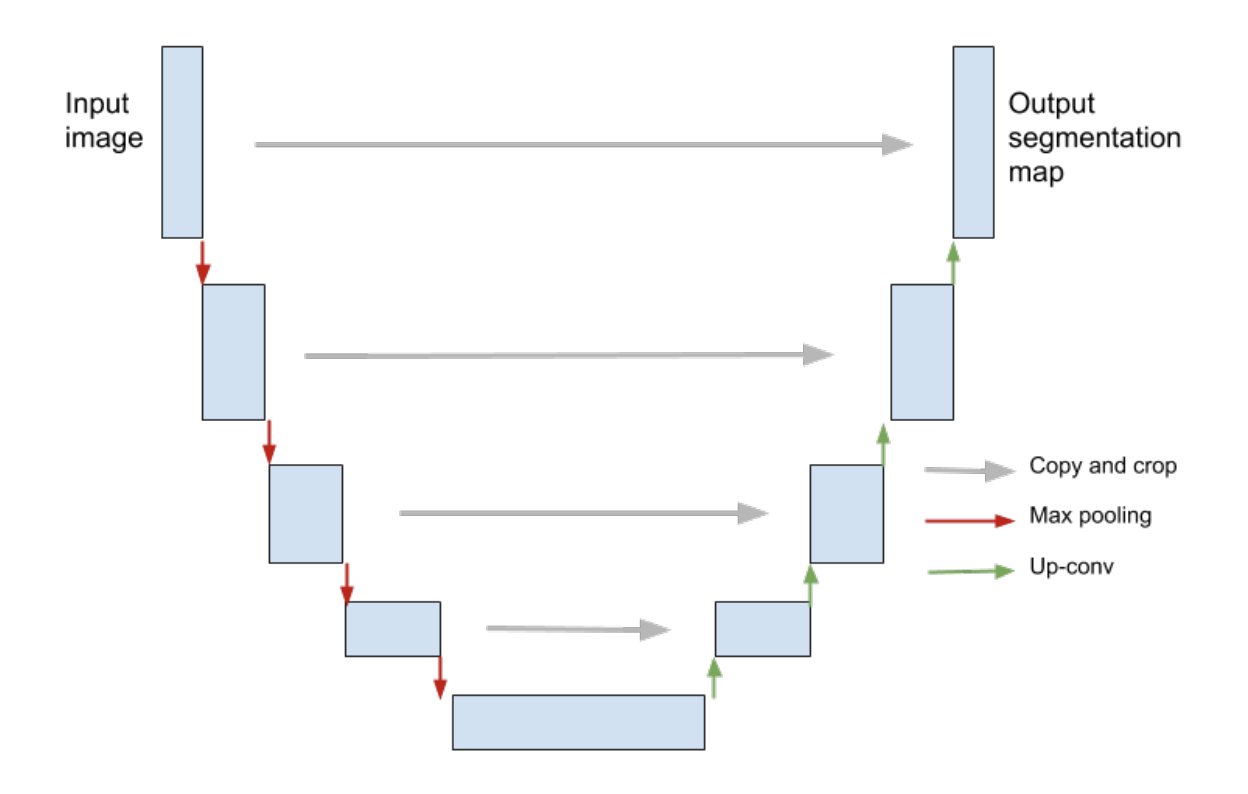
\includegraphics[width = 120mm]{images/unet.png}
	\caption{Architettura U-net.}
	\label{unet}
\end{figure}

Il percorso contrattuale dell'architettura di rete segue la struttura tipica di a rete convoluzionale. Ha l'applicazione ripetuta di strati convoluzionali seguiti da uno strato di pooling, che funge da operatore di downsampling \cite{ronneberger2015u}. A ciascuno fase di downsampling, il numero di mappe delle caratteristiche viene raddoppiato. Nell'espansivo percorso in cui il pool viene scambiato con gli operatori di sovracampionamento delle mappe delle caratteristiche. Questi aumenteranno la risoluzione dell'output. Per ottenere una maggiore precisione, Ronneberger et al [25], propongono una funzione di perdita ponderata. I pixel di sfondo separando due istanze della stessa classe si otterrà un peso maggiore nella perdita funzione, al fine di migliorare le separazioni degli oggetti adiacenti. Il metodo di base, che esegue la segmentazione semantica, è in questa tesi scelto come una rete U-net, con ResNet50 come spina dorsale. Questo dal momento che la rete l'architettura è simile al metodo attualmente utilizzato da Vricon come fase di estrazione delle impronte degli edifici.



\subsubsection{Semantic Segmentation}

\begin{figure}[htb]
	\centering
	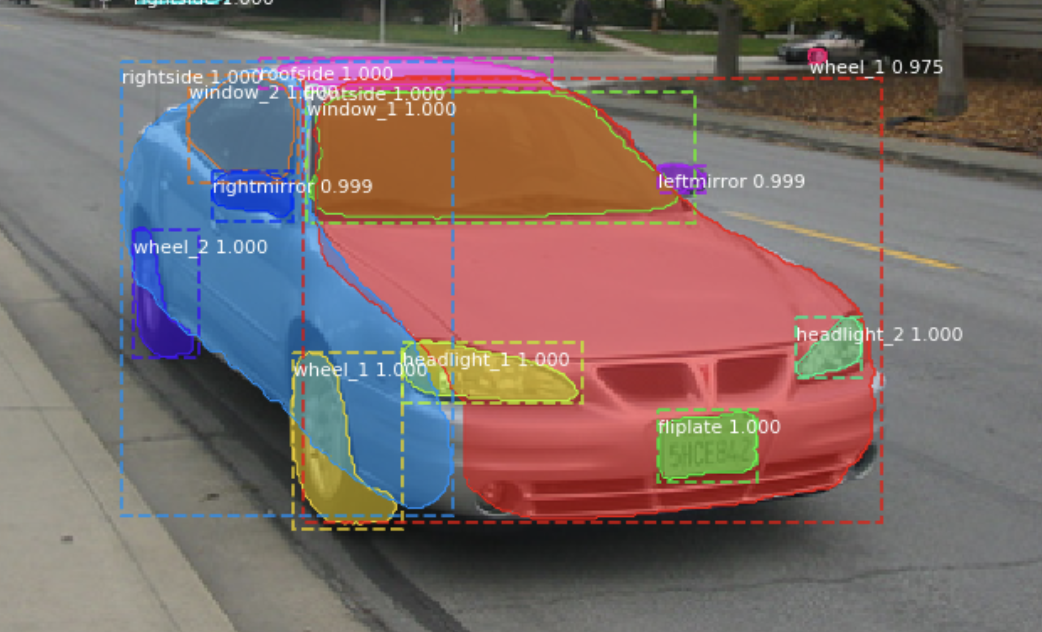
\includegraphics[width = 120mm]{images/car_seg.png}
	\caption{Task di segmentazione delle parti di un auto.}
	\label{car_seg}
\end{figure}


\subsubsection{Instance Segmentation}

Spinti dal successo delle proposte regionali nel rilevamento di oggetti, molti approcci per istanza la segmentazione si è basata su proposte di segmenti. Un esempio di un tale algoritmo è Deepmask [22], che è una rete che impara a proporre un segmento candidati, che vengono successivamente classificati con un algoritmo di rilevamento degli oggetti. Un altro metodo che utilizza le proposte di segmento è proposto da Dai et al [5], che esegue per primo il rilevamento di oggetti, da cui sono previste le proposte di segmento, che è poi seguita dalla classificazione. Successivamente, ogni proposta di segmento verrà classificata. Un altro esempio di una rete che esegue la segmentazione delle istanze è il Fully Segmentazione delle istanze convoluzionali, (FCIS). L'idea è di prevedere un insieme di canali di uscita sensibili alla posizione in modo completamente convoluzionale, che indirizzerà l'oggetto classi, scatole e maschere simultaneamente [10]. Per ottenere la segmentazione delle istanze con U-net, Iglovikov et al. [12], propone a metodo che aggiunge un canale di output extra dove confina tra gli oggetti che sono ravvicinati, o addirittura si toccano, sono previsti. Questo strato in seguito funge da una maschera e migliorerà la separazione degli oggetti. In questi casi, la segmentazione precede il riconoscimento [12]. La maschera r-cnn [10] è un altro metodo popolare sia per la segmentazione delle immagini che per rilevamento di oggetti. Il metodo è progettato per la segmentazione delle istanze e si basa sul modello di rilevamento di oggetti Faster R-CNN [24]. Oltre al rilevamento di oggetti e la predizione dei box di delimitazione, l'estensione da Faster r-cnn è un'ulteriore predizione di maschera binaria dell'oggetto all'interno del box di delimitazione [10]. Il il modello ha ottenuto risultati all'avanguardia sul set di dati MSCOCO [3], quando pubblicato. La scelta del metodo per la segmentazione delle istanze in questa tesi è Mask r-cnn, poiché questo è un metodo che esegue piuttosto la segmentazione delle istanze in parallelo che linearmente, il che rende il metodo diverso rispetto all'utilizzo di un'estensione di il metodo di base.








La instance segmentation ha l'obiettivo di assegnare un'etichetta a ciascun pixel in un'immagine (anche chiamata pixel-to-pixel classification). 

La Figura \ref{car_seg} illustra un'immagine di esempio dove sono state segmentate le componenti per la quale è stata addestrata, identificandole e localizzanodole all'interno della immagine a livello di pixel, differendosi per processo e per output dall'object detection visto in precedenza alla sezione \ref{cap:chapter2}. Esistono però due variazioni della segmentation che differiscono per numero massimo di istanze della stessa classe restituite, o per la shape del tensore di output.

\subsubsection{Mask rcnn}

Maschera r-cnn o mrcnn, estende Faster r-cnn aggiungendo un ramo che prevede una maschera oggetto in parallelo con il ramo utilizzato per la classificazione e il delimitazione box regressione. Ciò rende mrcnn in grado di combinare entrambe le parti classiche di rilevamento e segmentazione di oggetti [10]. Un'illustrazione semplificata della rete l'architettura è disponibile nella figura 2.5. Il ramo della maschera in mrcnn è un piccolo FCN, applicato a ciascun RoI, che esegue un previsione della maschera a livello di pixel. Questo è un classificatore binario poiché il modello dipende su questo le caselle proposte contengono solo un'istanza di una classe. Il predetto le proposte regionali sono come in Fast and Faster r-cnn rimodellate utilizzando il pooling RoI. RoIPool è un'operazione per estrarre mappe di piccole caratteristiche da ogni RoI. Da ogni regione è composta da numeri in virgola mobile, RoIPool prima quantizza il file regione a una mappa di caratteristiche discrete. Questa versione quantizzata verrà quindi suddivisa in contenitori spaziali, anch'essi quantizzati. I valori delle caratteristiche vengono quindi aggregati da max pooling. Queste quantizzazioni introducono disallineamenti tra il RoI e le caratteristiche estratte. Poiché la classificazione è robusta per le piccole traduzioni, questo non è un problema con r-cnn, ma avrà un grande impatto negativo sulla previsione di una maschera a livello di pixel poiché le caratteristiche del RoI devono essere ben allineate per conserva la corrispondenza spaziale per pixel. La soluzione è implementare un file tecnica chiamata RoI Align [10]. Il livello RoI Align rimuove la dura quantizzazione del pooling RoI e allinea le caratteristiche con l'input, che si è dimostrato per migliorare i risultati. RoI Align funziona evitando qualsiasi quantizzazione del RoI confini o contenitori. L'interpolazione bilineare viene utilizzata per calcolare i valori di inserire le caratteristiche in quattro posizioni regolarmente campionate in ogni bin RoI e aggregarle il risultato utilizzando il pooling massimo o medio [10].

\cite{he2017mask}

C'è qualche modo di utilizzare l'attuale rete per la segmentazione semantica? Ovviamente la risposta è stata sì. Ma invece della segmentazione semantica, loro ha proposto un approccio più avanzato, la segmentazione delle istanze. Implementare la segmentazione delle istanze con sufficiente precisione, era necessario apportare alcune modifiche all'architettura di Faster R-CNN. Seguendo la terminologia originale di [16], nella parte successiva, distinguerò tra l'architettura backbone per estrazione delle caratteristiche e architettura della testa per la classificazione, la regressione del riquadro di delimitazione e la previsione della maschera. Questi verranno descritti nelle parti seguenti di questo capitolo insieme a un focus extra su un RoIAlign, un nuovo approccio nella generazione di RoI